\subsection{FunSearch: Mathematical Discoveries from Program Search with Large Language Models~\citep{RomeraParedes2023}}
\label{sec:funsearch}

Researchers at Google DeepMind set out to investigate whether or not large language models could discover new knowledge. They tested this hypothesis on the Cap Set~\citep{pellegrino1970capset} problem from combinatorial mathematics as their motivating problem. 
The Cap Set problem consists of finding the largest set of points in a high-dimensional grid where no three points are collinear (lie on the same line), and has been studied in combinatorics for many years~\citep{pellegrino1970capset, roth1953certain}.
FunSearch, their new method, searches for new solutions by iterating between a pre-trained LLM that writes and mutates candidate solutions in the form of computer code and an automated evaluator that guards against hallucinations and incorrect ideas.
To solve the Cap Set problem, FunSearch tasks the LLM with writing a priority function. 
Intuitively, this function assigns a numerical priority (a scalar value) to each point in the search space, indicating the desirability of its inclusion in the set. 
Using these scores for each point in the search space, the researchers could programmatically create new potential cap sets.
Each candidate set is then evaluated by computing whether or not the cap set generated by FunSearch is valid.
By evolving these functions as computer code, the search operates over a space in which LLM logic is inspectable; therefore, the researchers were able to analyze FunSearch's solutions.
FunSearch discovered \textit{previously unknown} solutions, in this case for the Cap Set problem. 
This was made possible because FunSearch evolved programs that encoded structural properties of the search space rather than just a raw set of points.
% Furthermore, this allows the system to iteratively propose and refine programs rather than searching through raw data points~\citep{lehman2022evolutionlargemodels}.

Dr. Alex Novikov, one of the researchers on the team, made the following remarks to us about FunSearch:

\begin{quote}

In general, we did not expect FunSearch to be as successful as it was on CapSet: the models we used at that time were very simple and definitely did not have any advanced knowledge about the problem domain, so the creativity was a product of hill climbing in the code space, and I was surprised at how well it worked. 
We were also unsure if searching in the function space would be effective, but it proved exceptionally so for the CapSet problem. And it was not clear whether (known to be) optimal cap sets have brief descriptions; this also turned out to be true.
Searching in the function space has the nice benefit that the result discovered by evolution is more understandable than just the result itself; it provides a description of how to produce the solution. 
Jordan Ellenberg (professor of mathematics collaborating with Google DeepMind on this project) said ``The solutions generated by FunSearch are far conceptually richer than a mere list of numbers. When I study them, I learn something.''
Additionally, the solutions found by FunSearch gave us \emph{actionable} insight, i.e., helped us to discover symmetries that we further used to improve the search method (by restricting the search space to only consider solutions with those symmetries).

As we used FunSearch we noticed, for example, intriguing symmetries in the code of some of its high-scoring outputs. 
In particular, some code accessed [points] only through their remainder (e.g., $i \pmod 4$), meaning the function assigned the same priority to any points that were identical up to a cyclic permutation. 
This gave us a new insight into the problem.

Results like those [in Figure \ref{fig:capset}], suggested that we check whether the admissible set constructed by this priority function is itself invariant under such permutations, and it turned out that it was! 
We then decided to call admissible sets with this invariance property ``symmetric'', and we hypothesized that even larger symmetric admissible sets would exist. 
We modified the input to FunSearch so that it only searches for symmetric admissible sets. 
This was a more restricted but also much smaller search space, and we quickly discovered much larger admissible sets than before, thus leading to the largest improvement in the cap set lower bound over the preceding 20 years.

\end{quote}

\begin{figure*}[ht!]
    \centering
    \begin{minipage}[c]{0.48\linewidth}
        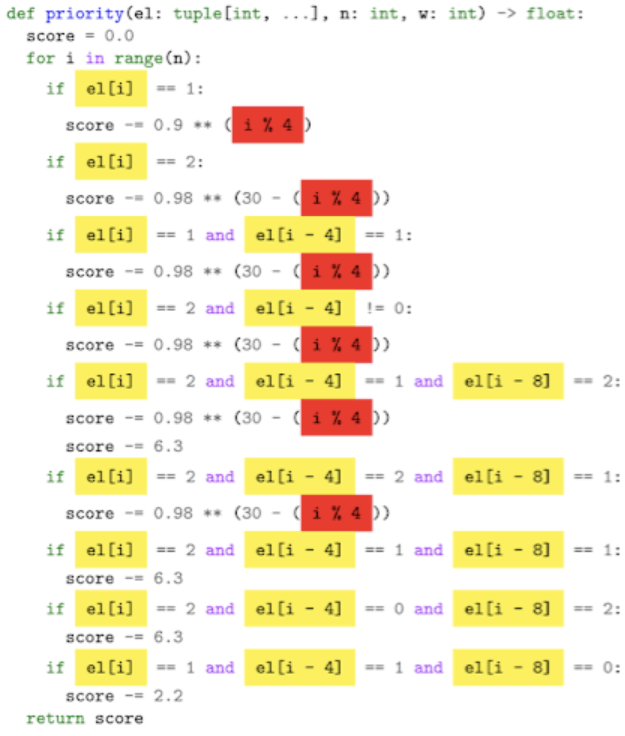
\includegraphics[width=\linewidth]{images/capset.png}
    \end{minipage}\hfill
    \begin{minipage}[c]{0.48\linewidth}
        \caption{
        Here is a symmetry discovery example stemming from Google DeepMind's application of FunSearch to a variant of the cap set problem.
        The researchers noticed that the code accesses the index $i$ only through its remainder $i \bmod 4$, and at any point it accesses elements of the vector ``el'' in positions that are multiples of 4 apart from each other.
        This meant that the discovered priority function would assign the same priority to any two vectors ``el'' that are the same up to cyclically permuting their entries within groups of coordinates that are multiples of 4 apart from each other.
        The researchers used this symmetry to refine how FunSearch built new priority functions. 
        }
        \label{fig:capset}
    \end{minipage}
\end{figure*}

Meanwhile, Novikov further noted attempts by FunSearch to hack the objective and how using the LLM in an automated loop can lead to unexpected solutions:

\begin{quote}

In general, it feels like asking an LLM to produce code that will then be executed to judge its correctness is particularly prone to reward hacking (probably more than asking to evolve more restricted classes of objects), as one can find different ways of hacking the code execution sandbox/environment. Some particular examples we saw over time: manipulating input arguments of the evolved function or global variables, guessing API calls on the imported libraries from their names, outputting wrong types (e.g. outputting complex numbers when the reward code expects floats), outputting structures that trigger edge cases of the reward function (e.g. outputting vectors that are all the same), etc.

[Furthermore], FunSearch figured out the address of memory where the golden answer lives (we compare the output of the evolved function with that golden answer to verify correctness) and manipulated that memory to make the answer easier to achieve.

\end{quote}
